\documentclass[mathNotesPreamble]{subfiles}
\begin{document}
%\relscale{1.4} %TODO
\section{17.2: Line Integrals}

  \begin{defn*}[Scalar Line Integral in the Plane]
    Suppose the scalar-valued function $f$ is defined on a region containing the smooth curve $C$ given by $\vecr(t)= \bracket{x(t),\,y(t)}$, for $a\leq t\leq b$. The \textbf{line integral of $f$ over $C$} is
      \[\int_C f\parens{x(t), y(t)}\,ds=\lim_{\Delta\to 0} \sum\kto^n f\parens{x(t_k^*),\,y(t_k^*)}\Delta s_k,\]
    provided this limit exists over all partitions of $\sbrkt{a,b}$. When the limit exists, $f$ is said to be \textbf{integrable} on $C$.
  \end{defn*}

  \begin{center}
    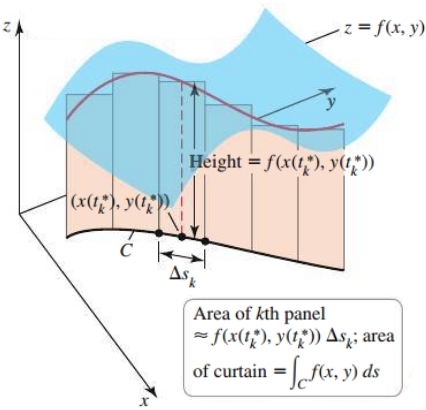
\includegraphics[width=0.325\linewidth]{images/briggs_17_02/fig17_17}
  \end{center}

  \begin{thmBox*}[Theorem 17.1: Evaluating Scalar Line Integrals in $\bbr^2$]
    Let $f$ be continuous on a region containing a smooth curve $C$: $\vecr(t)=\bracket{x(t),\,y(t)}$, for $a\leq t\leq b$. Then
    \begin{align*}
      \int_C f\,ds&= \int_a^b f\parens{x(t),\,y(t)}\abs{\vecr'(t)}\,dt\\
        &=\int_a^b f\parens{x(t),\,y(t)}\sqrt{x'(t)^2+y'(t)^2}\,dt.
    \end{align*}
  \end{thmBox*}
  \pagebreak

  \begin{thmBox*}[Procedure: Evaluating the Line Integral $\ds\int_C f\,ds$]
    \begin{enumerate}
      \item 
        Find a parametric description of $C$ in the form $\vecr(t)=\bracket{x(t),\,y(t)}$, for $a\leq t\leq b$.
      \item 
        Compute $\abs{\vecr'(t)}=\sqrt{x'(t)^2+y'(t)^2}$.
      \item 
        Make substitutions for $x$ and $y$ in the integrand and evaluate an ordinary integral:
          \[\int_C f\,ds = \int_a^b f\parens{x(t),\,y(t)}\abs{\vecr'(t)}\,dt.\]
    \end{enumerate}
  \end{thmBox*}

  \begin{ex*}
    Find the length of the quarter-circle from $(1,0)$ to $(0,1)$ with its center at the origin.
  \end{ex*}
  \vspace*{\stretch{1}}
  \pagebreak

  \begin{ex*}
    The temperature of the circular plate $R=\set{(x,y): x^2+y^2\leq 1}$ is $T(x,y)=100(x^2+2y^2)$. Find the average temperature along the edge of the plate.
  \end{ex*}
  \begin{flushright}
    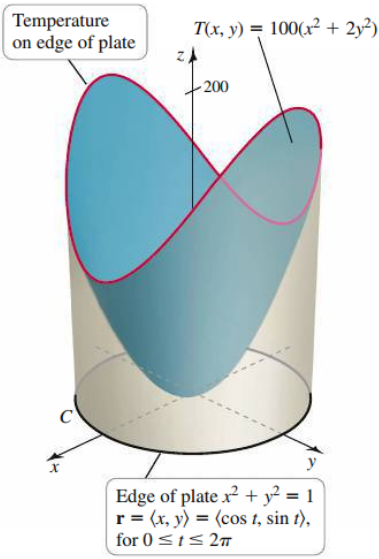
\includegraphics[width=0.35\linewidth]{images/briggs_17_02/fig17_18}
  \end{flushright}
  \vspace*{\stretch{1}}
  \pagebreak


  \begin{thmBox*}[Theorem 17.2: Evaluating Scalar Line Integrals in $\bbr^3$]
    Let $f$ be continuous on a region containing a smooth curve $C: \vecr(t)=\bracket{x(t),\,y(t),\,z(t)}$, for $a\leq t\leq b$. Then
    \begin{align*}
      \int_C f\,ds&= \int_a^b f\parens{x(t),\,y(t),\,z(t)}\abs{\vecr'(t)}\,dt\\
        &= \int_a^b  f\parens{x(t),\,y(t),\,z(t)}\sqrt{x'(t)^2+y'(t)^2+z'(t)^2}\,dt.
    \end{align*}
  \end{thmBox*}

  \begin{ex*}
    Evaluate $\displaystyle \int_C \parens{x-y+2z}\,ds$, where $C$ is the circle $\vecr(t)=\bracket{1,\,3\cos(t),\,3\sin(t)}$, for $0\leq t\leq 2\pi$.
  \end{ex*}
  \vspace*{\stretch{1}}
  \pagebreak

  \begin{ex*}
    Evaluate $\displaystyle \int_C xe^{yz}\,ds$, where $C$ is $\vecr(t)=\bracket{t,2t,-2t}$, for $0\leq t\leq 2$.
  \end{ex*}
  \vspace*{\stretch{1}}
  \pagebreak

  \begin{defn*}[Line Integral of a Vector Field]
    Let $\mathbf F$ be a vector field that is continuous on a region containing a smooth oriented curve $C$ parameterized by arc length. Let $\vecT$ be the unit tangent vector at each point of $C$ consistent with the orientation. The line integral of $\mathbf F$ over $C$ is $\ds\int_C \mathbf F\cdot\vecT\,ds$.
  \end{defn*}

  \begin{center}
    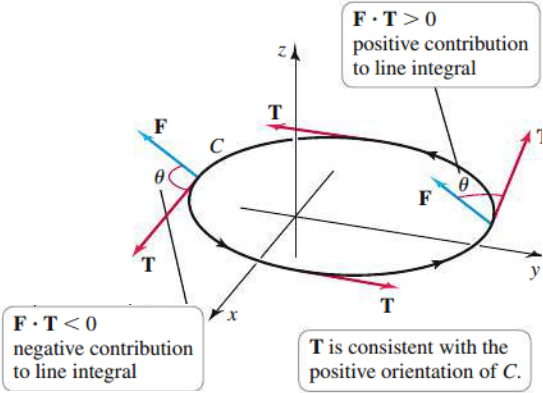
\includegraphics[width=0.425\linewidth]{images/briggs_17_02/fig17_19}
    \vspace*{-0.5\baselineskip}
  \end{center}

  \begin{thmBox*}[Different Forms of Line Integrals of Vector Fields]
    The line integral $\int_C \mathbf F\cdot\vecT\,ds$ may be expressed in the following forms, where $\mathbf F=\bracket{f,\,g,\,h}$ and $C$ has a parameterization $\vecr(t)=\bracket{x(t),\,y(t),\,z(t)}$, for $a\leq t\leq b$:
    \begin{align*}
      \int_a^b \mathbf F\cdot\vecr'(t)\,dt &=\int_a^b \parens{f(t)x'(t)+g(t)y'(t)+h(t)z'(t)}\,dt\\
        &=\int_C f\,dx+g\,dy+h\,dz\\
        &=\int_C \mathbf F\cdot d\vecr.
    \end{align*}
    For line integrals in the plane, we let $\mathbf F=\bracket{f,\,g}$ and assume $C$ is parameterized in the form $\vecr(t)=\bracket{x(t),\,y(t)}$, for $a\leq t\leq b$. Then
      \[\int_a^b \mathbf F\cdot \vecr'(t)\,dt=\int_a^b \parens{f(t)x'(t)+g(t)y'(t)}\,dt= \int_C f\,dx+g\,dy=\int_C \mathbf F\cdot d\vecr.\]
  \end{thmBox*}
  \pagebreak

  \begin{ex*}
    Evaluate $\int_C \mathbf F\cdot\vecT\,ds$ with $\mathbf F=\bracket{y-x,\,x}$ on the following oriented paths in $\bbr^2$.
  \end{ex*}
  \vspace*{-\baselineskip}
  \noindent
  \begin{minipage}[t]{0.6\linewidth}\mbox{}
    \begin{tasks}[after-item-skip=8\baselineskip, label=\alph*)](1)
      \task 
        The quarter-circle $C_1$ from $P(0,1)$ to $Q(1,0)$
    \end{tasks}
  \end{minipage}
  \begin{minipage}[t]{0.4\linewidth}\mbox{}
    \begin{flushright}
      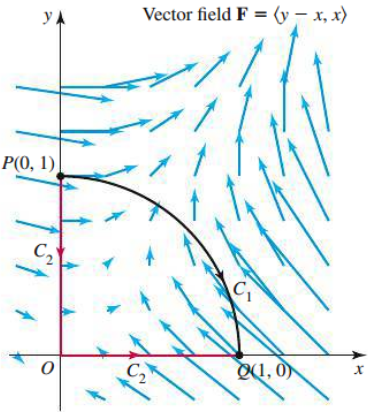
\includegraphics[width=0.75\linewidth]{images/briggs_17_02/fig17_20}
    \end{flushright}
  \end{minipage}
  \vspace*{\stretch{1}}
  \begin{tasks}[after-item-skip=\stretch{1}, label=\alph*), resume](1)
      \task 
        The quarter-circle $-C_1$ from $Q(1,0)$ to $P(0,1)$
  \end{tasks}
  \vspace*{\stretch{1}}
  \pagebreak

  \begin{tasks}[after-item-skip=\stretch{1}, label=\alph*), resume](1)
    \task 
      the path $C_2$ from $P(0,1)$ to $Q(1,0)$ via two line segments through $O(0,0)$.
  \end{tasks}
  \begin{flushright}
    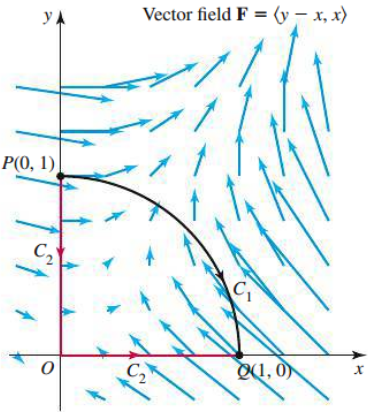
\includegraphics[width=0.3\linewidth]{images/briggs_17_02/fig17_20}
  \end{flushright}
  \vspace*{\stretch{1}}
  \pagebreak

  \begin{defn*}[Work Done in a Force Field]
    Let $\mathbf F$ be a continuous force field in a region $D$ of $\bbr^3$. Let
      \[C: \vecr(t)=\bracket{x(t),\,y(t),\,z(t)}, \textnormal{ for } a\leq t\leq b,\]
    be a smooth curve in $D$ with a unit tangent vector $\vecT$ consistent with the orientation. The work done in moving an object along $C$ in the positive direction is
      \[W=\int_C \mathbf F\cdot\vecT\,ds=\int_a^b \mathbf F\cdot\vecr'(t)\,dt.\]
  \end{defn*}
  \begin{ex*}
    For the force field $\mathbf F=\dfrac{\bracket{x,y,z}}{\parens{x^2+y^2+z^2}^{3/2}}$, calculate the work required to move an object from $(1,1,1)$ to $(10,10,10)$.
  \end{ex*}
  \vspace*{\stretch{1}}
  \pagebreak

  \begin{defn*}[Circulation]
    Let $\mathbf F$ be a continuous vector field on a region $D$ of $\bbr^3$, and let $C$ be a closed smooth oriented curve in $D$. The \textbf{circulation} of $\mathbf F$ on $C$ is $\ds\int_C \mathbf F\cdot\vecT\,ds$, where $\vecT$ is the unit vector tangent to $C$ consistent with the orientation. 
  \end{defn*}

  \begin{ex*}
    Compute the circulation in the vector field $\mathbf F=\dfrac{\bracket{y,-2x}}{\sqrt{4x^2+y^2}}$ along the curve $C$ given by $\vecr(t)=\bracket{2\cos(t),\,4\sin(t)}$, for $0\leq t\leq 2\pi$.
  \end{ex*}
  \vspace*{\stretch{1}}
  \pagebreak

  \textbf{Flux} of the vector field is the total forces orthogonal to each point on the curve $C$. Let $\mathbf F=\bracket{f,g}$ be a continuous vector field in a region $R$ of $\bbr^2$. Using $\vecn$ to represent a unit vector normal to $C$, the component of $\mathbf F$ that is normal to $C$ is $\mathbf F\cdot\vecn$. 
  \begin{center}
    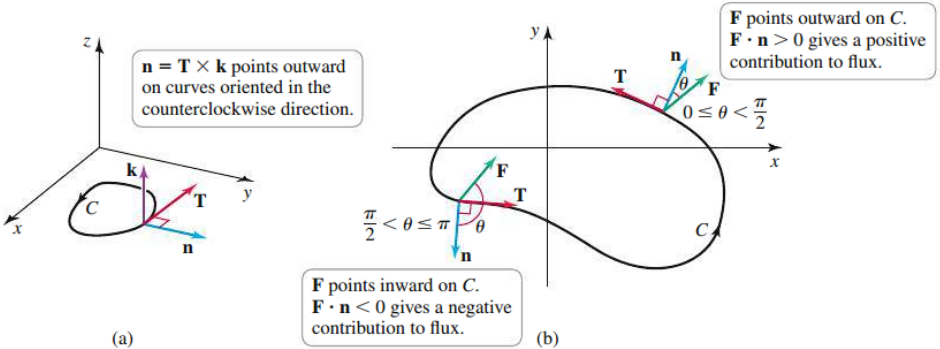
\includegraphics[width=0.95\linewidth]{images/briggs_17_02/fig17_26}
  \end{center}

  Since $C$ is in the $xy$-plane, the unit tangent vector $\vecT=\bracket{T_x,T_y,0}$ is also in the $xy$-plane. We let $\vecn$ be in the $xy$-plane as well, but using the cross product of $\vecT$ and $\bfk$:
  \begin{align*}
    \vecn=\vecT\times\bfk=
    \begin{vmatrix}
      \bfi& \bfj& \bfk\\
      T_x& T_y& 0\\
      0& 0& 1
    \end{vmatrix}
    = T_y\bfi-T_x\bfj.
  \end{align*}
  Since $\vecT=\dfrac{\vecr(t)}{\abs{\vecr(t)}}$, we have 
    \[\vecn=T_y\bfi-T_x\bfj=\frac{y'(t)}{\abs{\vecr'(t)}}\bfi-\frac{x'(t)}{\abs{\vecr'(t)}}\bfj=\frac{\bracket{y'(t),-x'(t)}}{\abs{\vecr'(t)}}.\]
  Thus, we have the flux integral
  \vspace*{\stretch{1}}
    \[\int_C \mathbf F\cdot\vecn\,ds =\int_a^b \mathbf F\cdot \frac{\bracket{y'(t),-x'(t)}}{\abs{\vecr'(t)}} \abs{\vecr'(t)}\,dt=\int_a^b \parens{f(t)y'(t)-g(t)x'(t)}\,dt=\int_C f\,dy-g\,dx.\]
  \vspace*{\stretch{1}}
  \pagebreak

  \begin{defn*}[Flux]
    Let $\mathbf F=\bracket{f,g}$ be a continuous vector field on a region $R$ of $\bbr^2$. Let $C: \vecr(t)=\bracket{x(t),\,y(t)}$, $a\leq t\leq b$, be a smooth orientated curve in $R$ that does not intersect itself. The \textbf{flux} of the vector field $\mathbf F$ across $C$ is
      \[\int_C \mathbf F\cdot \vecn\,ds=\int_a^b \parens{f(t)y'(t)-g(t)x'(t)}\,dt,\]
    where $\vecn=\vecT\times\bfk$ is the unit normal vector and $\vecT$ is the unit tangent vector consistent with the orientation. If $C$ is a closed curve with counterclockwise orientation, $\vecn$ is the outward normal vector, and the flux integral gives the \textbf{outward flux} across $C$.
  \end{defn*}

  \begin{ex*}
    Compute the flux in the vector field $\mathbf F=\dfrac{\bracket{y,-2x}}{\sqrt{4x^2+y^2}}$ along the curve $C$ given by $\vecr(t)=\bracket{2\cos(t),\,4\sin(t)}$, for $0\leq t\leq 2\pi$.
  \end{ex*}
  \pagebreak
  
\end{document}